% =============================================================================
% COPYRIGHT AND DISCLAIMER
% =============================================================================
% This file is provided as a convenience template for competition participants.
% By using it, you accept full responsibility for compliance with all applicable
% copyright, licensing, and usage rules of the Association for Computing
% Machinery (ACM) and of any LaTeX packages you load (including, without
% limitation, the "acmart" document class and related ACM materials).
%
% Consult ACM's official publication, template, and copyright policies before
% using this setup for any purpose other than this competition. Do not assume
% that this template may be reused, redistributed, or submitted elsewhere
% without independently verifying ACM's current rules.
%
% Use of the "acmart" class, the "sigconf" option, or ACM-style formatting in
% this template does NOT mean that this report, this competition, its organizers,
% or any resulting PDF is sponsored, endorsed, affiliated with, or published by
% ACM. ACM trademarks and branding remain the property of ACM.
%
% Template packages live in preamble.tex.
% Citations live in main.bib. Edit this file with your paper content.
% =============================================================================

\documentclass[sigconf]{acmart}
% =============================================================================
% Template setup — participants normally do not edit this file.
% Author content belongs in main.tex; citations belong in main.bib.
% \documentclass lives in main.tex so Overleaf does not treat this file as root.
% =============================================================================

% --- Competition / non-ACM-submission friendly rights metadata -------------
\setcopyright{none}
\settopmatter{printacmref=false}
\acmConference[Kaggle Competition]{Filament Segmentation Challenge}{2026}{\href{https://www.kaggle.com/competitions/filament-segmentation-2026}{kaggle.com/competitions/filament-segmentation-2026}}
\acmBooktitle{Competition Report}
\acmDOI{}
\acmISBN{}

% --- Author guidance text --------------------------------------------------
% \guide{...} is gray italic while \guideStyletrue; omitted from the PDF if false.
% Flip the switch in main.tex after % =============================================================================
% Template setup — participants normally do not edit this file.
% Author content belongs in main.tex; citations belong in main.bib.
% \documentclass lives in main.tex so Overleaf does not treat this file as root.
% =============================================================================

% --- Competition / non-ACM-submission friendly rights metadata -------------
\setcopyright{none}
\settopmatter{printacmref=false}
\acmConference[Kaggle Competition]{Filament Segmentation Challenge}{2026}{\href{https://www.kaggle.com/competitions/filament-segmentation-2026}{kaggle.com/competitions/filament-segmentation-2026}}
\acmBooktitle{Competition Report}
\acmDOI{}
\acmISBN{}

% --- Author guidance text --------------------------------------------------
% \guide{...} is gray italic while \guideStyletrue; omitted from the PDF if false.
% Flip the switch in main.tex after % =============================================================================
% Template setup — participants normally do not edit this file.
% Author content belongs in main.tex; citations belong in main.bib.
% \documentclass lives in main.tex so Overleaf does not treat this file as root.
% =============================================================================

% --- Competition / non-ACM-submission friendly rights metadata -------------
\setcopyright{none}
\settopmatter{printacmref=false}
\acmConference[Kaggle Competition]{Filament Segmentation Challenge}{2026}{\href{https://www.kaggle.com/competitions/filament-segmentation-2026}{kaggle.com/competitions/filament-segmentation-2026}}
\acmBooktitle{Competition Report}
\acmDOI{}
\acmISBN{}

% --- Author guidance text --------------------------------------------------
% \guide{...} is gray italic while \guideStyletrue; omitted from the PDF if false.
% Flip the switch in main.tex after \input{preamble}.
%
% Do not use \guide{...} for \email{...}.
\usepackage{xcolor}
\newif\ifguideStyle
\guideStyletrue
\newcommand{\guide}[1]{%
  \ifguideStyle
    {\color{gray!65}\itshape #1}%
  \fi
}

% --- Math ------------------------------------------------------------------
% Do NOT load amssymb (or amsfonts): acmart already loads newtxmath, which
% defines the same symbols (e.g. \Bbbk) and causes a conflict on Overleaf.
% amsmath is already provided by acmart; mathtools extends it.
\usepackage{mathtools}

% --- Figures ---------------------------------------------------------------
% graphicx is already loaded by acmart
\usepackage{subcaption}

% --- Tables ----------------------------------------------------------------
% booktabs is already loaded by acmart
\usepackage{tabularx}
\usepackage{multirow}

% --- Bibliography style is set in main.tex (ACM-Reference-Format) ----------
.
%
% Do not use \guide{...} for \email{...}.
\usepackage{xcolor}
\newif\ifguideStyle
\guideStyletrue
\newcommand{\guide}[1]{%
  \ifguideStyle
    {\color{gray!65}\itshape #1}%
  \fi
}

% --- Math ------------------------------------------------------------------
% Do NOT load amssymb (or amsfonts): acmart already loads newtxmath, which
% defines the same symbols (e.g. \Bbbk) and causes a conflict on Overleaf.
% amsmath is already provided by acmart; mathtools extends it.
\usepackage{mathtools}

% --- Figures ---------------------------------------------------------------
% graphicx is already loaded by acmart
\usepackage{subcaption}

% --- Tables ----------------------------------------------------------------
% booktabs is already loaded by acmart
\usepackage{tabularx}
\usepackage{multirow}

% --- Bibliography style is set in main.tex (ACM-Reference-Format) ----------
.
%
% Do not use \guide{...} for \email{...}.
\usepackage{xcolor}
\newif\ifguideStyle
\guideStyletrue
\newcommand{\guide}[1]{%
  \ifguideStyle
    {\color{gray!65}\itshape #1}%
  \fi
}

% --- Math ------------------------------------------------------------------
% Do NOT load amssymb (or amsfonts): acmart already loads newtxmath, which
% defines the same symbols (e.g. \Bbbk) and causes a conflict on Overleaf.
% amsmath is already provided by acmart; mathtools extends it.
\usepackage{mathtools}

% --- Figures ---------------------------------------------------------------
% graphicx is already loaded by acmart
\usepackage{subcaption}

% --- Tables ----------------------------------------------------------------
% booktabs is already loaded by acmart
\usepackage{tabularx}
\usepackage{multirow}

% --- Bibliography style is set in main.tex (ACM-Reference-Format) ----------


% Guide styling: \guideStyletrue = show gray italic hints; \guideStylefalse = omit them
% \guideStyletrue
\guideStylefalse

\begin{document}

\title{Propose, Refine and Merge: A Cascade for Solar Filament Instance Segmentation}
\subtitle{A Solution to the Solar Filament Segmentation Challenge 2026} % DO NOT CHANGE


% TODO: fill in every author's surname, institution, city, country and email.
\author{Richmond Azumah}
\affiliation{%
  \institution{TODO Institution}
  \city{TODO City}
  \country{TODO Country}
}
\email{first.author@example.com}   % <- Replace with your own email

\author{Charan TODO}
\affiliation{%
  \institution{TODO Institution}
  \city{TODO City}
  \country{TODO Country}
}
\email{second.author@example.com}  % <- Replace with your own email

\author{Hassan TODO}
\affiliation{\institution{TODO Institution}\city{TODO City}\country{TODO Country}}
\email{third.author@example.com}

\author{Sheikh TODO}
\affiliation{\institution{TODO Institution}\city{TODO City}\country{TODO Country}}
\email{fourth.author@example.com}

\author{Varshi TODO}
\affiliation{\institution{TODO Institution}\city{TODO City}\country{TODO Country}}
\email{fifth.author@example.com}

% \author{\guide{Second Author}}
% \affiliation{%
%   \institution{\guide{Your Institution}}  % <- Optional (remove if you are not currently affiliated with any institute)
%   \city{\guide{City}}
%   \country{\guide{Country}}
% }
% \email{second.author@example.com}  % <- Replace with your own email

\begin{abstract}
    This report describes our solution to the Solar Filament Segmentation Challenge~2026, a Kaggle competition on automatic segmentation of solar filaments in GONG H-$\alpha$ observations. Our pipeline has three learned stages:
    a YOLO11l-seg instance proposer, a ConvNeXt U-Net whose filament and centerline probabilities guide the
    next stage, and an instance-conditioned ResNet-34 refiner that redraws each proposal's mask and predicts
    its own IoU. A second U-Net trained at native resolution supplies extra proposals that are refined the
    same way and merged by score-ranked overlap resolution. On a leak-free 5-fold out-of-fold evaluation over
    all 707 training images the final system reaches Panoptic Quality 0.460 (95\% CI 0.451--0.468), against
    0.421 for YOLO alone and 0.344 for one human annotator scored against the others; it scores 0.40 on the
    public leaderboard.
\end{abstract}

\maketitle

\ifguideStyle
\noindent{\color{gray!65}\itshape
Guide mode is on.}
\par\medskip
\fi

\guide{Please limit your report to four (4) pages, excluding the Acknowledgment and References sections. Throughout this document, please follow these considerations: 
\begin{itemize}
    \item Do not alter any text that is currently in black color (except for the emails under authors' name).
    \item Replace all gray text with your own.
    \item When you are done with the report, please replace \texttt{\textbackslash guideStyletrue} with \texttt{\textbackslash guideStylefalse}, to remove any gray text. Alternatively, you can remove any text wrapped in \texttt{\textbackslash guide\{\}},
    \item Be as succinct as possible, and only provide details regarding your own work. For example, there is no need to discuss what solar filaments are, or why filament segmentation matters.
    \item If you must, you can add extra sections.
\end{itemize}}


% ==================================== %
%              INTRODUCTION            %
% ==================================== %
\section{Introduction}
    This report goes over the details of our submitted solution to the Solar Filament Segmentation Challenge~2026 \cite{filament-segmentation-2026}. The challenge, launched on July~10,~2026, is organized by the Earth-Space AI Research (ESAIR) Lab\footnote{\href{https://www.esairlab.com/home}{www.esairlab.com/}}. This challenge utilizes the MAGFiLO dataset for evaluation of the segmentation algorithms \cite{ahmadzadeh2024dataset}. The training set has 707 full-disk images at
    2048$\times$2048 px with 1 to 3 independent annotation sets each (1,154 sets, 8,199 filament polygons);
    the test set has 180 images. Submissions are scored with Panoptic Quality~\cite{kirillov2019panoptic},
    $\mathrm{PQ}=\sum_{\mathrm{TP}}\mathrm{IoU}/(|\mathrm{TP}|+\tfrac12|\mathrm{FP}|+\tfrac12|\mathrm{FN}|)
    =\mathrm{SQ}\times\mathrm{RQ}$, where a prediction matches a filament when their IoU exceeds 0.5.

    Filament segmentation moved from thresholding and morphology~\cite{qu2005automatic} to deep networks:
    U-Nets on full-disk H$\alpha$ images~\cite{zhu2019solar, zhu2025flat}, Mask R-CNN for filament
    instances~\cite{ahmadzadeh2019toward}, and detection followed by segmentation, where YOLO boxes on
    ChroTel and GONG images supervise a U-Net~\cite{diercke2024universal}; see~\cite{butka2026survey} for
    a survey of deep learning on solar structures. Most of this work scores pixel masks (Dice, IoU), while
    PQ also rewards separating and counting individual filaments. A two-stage solution to this challenge,
    YOLO11m boxes followed by a UNet++ crop segmenter, reports validation PQ 0.415 and public PQ
    0.37~\cite{ghosh2026twostage}.

    Annotators disagree strongly: one annotator scored against the others reaches only PQ 0.344. A
    single detector therefore faces two problems at once: drawing tight masks around thin, faint structures
    (segmentation quality) and deciding which candidates most annotators would draw (recognition quality).
    Our design separates them: a detector proposes generously, a refiner redraws each candidate and
    estimates its quality, and a second, differently trained proposer recovers filaments the first one
    misses. Only the provided images are used at inference, and the JSON spine and chirality fields are never
    used; centerlines are derived by skeletonizing masks. Code, pinned requirements, fp16 weights and an
    end-to-end notebook: \url{https://github.com/hsfcoulibaly/aml_project} (directory \texttt{Azumah/}).



% ==================================== %
%              METHODOLOGY             %
% ==================================== %
\section{Methodology}\label{sec:methodology}
    Figure~\ref{fig:pipe} shows the end-to-end pipeline. Every learned stage is trained five times, once
    per held-out fold, plus once on all data; on the test set the fold models and the full model are used
    together.

\begin{figure}[t]
  \centering
  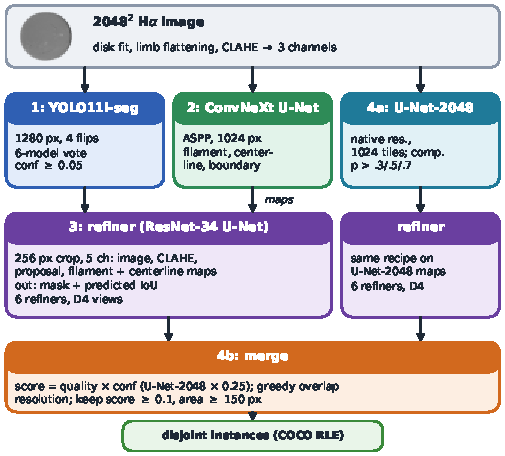
\includegraphics[width=\columnwidth]{pipeline_column.pdf}
  \caption{End-to-end pipeline: preprocessing, two proposal sources (YOLO11l-seg and a native-resolution
    U-Net), the instance-conditioned refiner guided by U-Net maps, and the score-ranked merge.}
  \Description{Block diagram of the pipeline from the input image through two proposal branches and refiners to the merged instance masks.}
  \label{fig:pipe}
\end{figure}

\subsection{Pre-processing and targets}
    We fit the solar disk, divide out radial limb darkening and stack the raw, limb-flattened and
    CLAHE~\cite{zuiderveld1994clahe} images as three channels, with the sky set to zero.
    Keeping the raw image next to the flattened one leaves the photometric context to the network, since
    fixed normalization alone can remove useful signal for filament segmentation~\cite{stepanyuk2026datadriven}. Instances from
    different annotation sets of an image are clustered (IoU $>0.2$ or $>50\%$ cover); a consensus target
    keeps a filament drawn by at least half of the image's annotators.

\subsection{Sampling and validation}
    All annotation sets of a physical image stay in one fold. We use 5 folds stratified by observing site
    and filament-count quartile (141--142 images each). Grouping by image does not remove temporal
    leakage~\cite{stepanyuk2026datadriven}: about a quarter of validation images have a training image
    taken within 24 hours, so OOF scores are mildly optimistic. Every number in
    Section~\ref{sec:evaluation} is out-of-fold (OOF): each image is predicted by models that never saw it, and post-processing thresholds
    are tuned once on the pooled 707 images. Tuning on a single fold was 0.004 PQ optimistic, and the public
    leaderboard (two decimals, about 90 images) cannot separate variants within 0.01, so pooled OOF PQ drives
    every design decision.

\subsection{Stage 1: YOLO proposals}
    YOLO11l-seg~\cite{yolo11} (27.6M parameters, COCO-pretrained, one class) is trained on the consensus
    targets at 1280 px (median filament width is about 11 px at 2048) for 60 epochs with AdamW, a cosine
    schedule, 180$^\circ$ rotations, flips and mosaic. Inference merges 4 flip views by mask voting; on the
    test set the 5 fold models and the full model vote. Every instance with confidence $\ge 0.05$ is kept,
    so the later stages decide what survives.

\subsection{Stage 2: dense U-Net maps}
    A U-Net~\cite{ronneberger2015unet} with a ConvNeXt-tiny~\cite{liu2022convnext} encoder and a residual
    ASPP block~\cite{chen2017deeplab} sees the whole disk at 1024 px and predicts three maps: filament (soft
    target equal to the fraction of annotators marking each pixel), centerline (dilated skeletons) and
    boundary. The loss combines weighted BCE, batch soft Dice and clDice~\cite{shit2021cldice} on the
    filament map, plus BCE on the centerline and boundary maps.

\subsection{Stage 3: instance-conditioned refiner}
    The refiner follows the two-stage idea of Mask R-CNN~\cite{he2017maskrcnn} and of crop segmenters for
    this task~\cite{ghosh2026twostage}, but is conditioned on the proposal itself and scores its own output.
    For each proposal we crop a square around its box with 1.5$\times$ context, resize it to 256 px and
    stack five channels: two image channels, the proposal mask, and the U-Net filament and centerline
    probabilities. A U-Net with a ResNet-34~\cite{he2016resnet} encoder (Segmentation Models
    PyTorch~\cite{iakubovskii2019smp}) redraws the mask, and a scalar head predicts the IoU of that mask with
    the matched filament (0 for false positives). Training mixes three kinds of samples: ground-truth
    filaments with a corrupted copy as the prior (down-up sampling, erosion, dilation, shifts, dropped
    segments, bleeding into neighbours), real OOF YOLO proposals matched at IoU $>0.2$, and unmatched
    proposals as negatives with an empty target. The loss is BCE + Dice on the mask and smooth L1 on the
    quality; we train 60 epochs and use all 8 dihedral (D4) views at test time. Each refined instance is
    scored by predicted quality $\times$ YOLO confidence.

\subsection{Stage 4: second proposal source and merge}
    YOLO misses about a third of the filaments. A second U-Net with the same architecture, trained at native
    2048 px on 1024 px crops, is cut into connected components at probabilities 0.3, 0.5 and 0.7 (near
    duplicates removed); each component is refined by a second set of refiners trained with the same recipe
    on these maps. Both refined sets are ranked by score, with the second source multiplied by $w=0.25$,
    and resolved greedily: an instance is dropped when less than half of it remains uncovered by
    higher-ranked ones. We keep instances with score $\ge 0.1$ and area $\ge 150$ px. Figure~\ref{fig:qual}
    shows example segmentations.

\begin{figure*}[t]
  \centering
  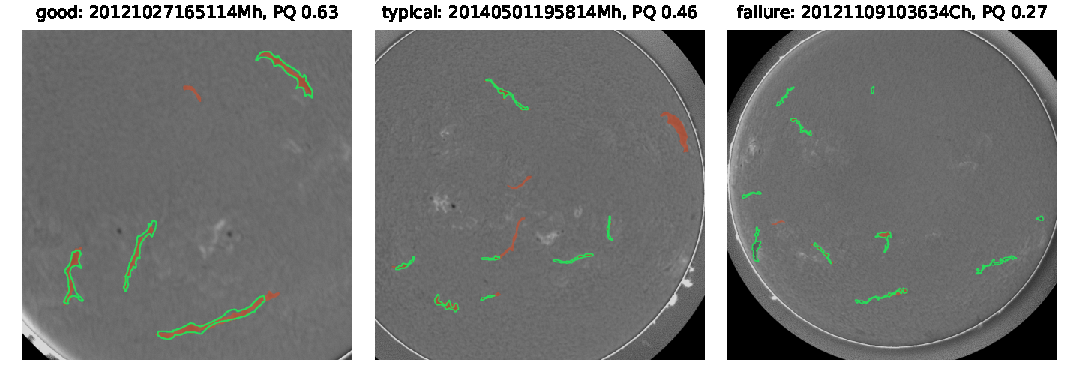
\includegraphics[width=0.85\textwidth]{fig_qualitative.pdf}
  \caption{Final model on OOF images at the 95th, 50th and 5th percentile of per-image PQ (among images
    with at least 4 filaments). Red: predictions; green outline: first annotation set (PQ averages over all
    sets).}
  \Description{Three cropped solar disk images with predicted filaments filled in red and annotated filaments outlined in green.}
  \label{fig:qual}
\end{figure*}

% ==================================== %
%              EVALUATION              %
% ==================================== %
\section{Evaluation}\label{sec:evaluation}
\subsection{Strategy}
    Because a hidden test label is one annotator's set, we score every image against each of its annotation
    sets and average, which estimates the expected leaderboard PQ. We also report the share of ground-truth
    filaments split across two or more predictions (one-to-many, fragmentation) and the share of predictions
    that swallow two or more filaments (many-to-one, over-merging). Uncertainty is given as 95\% bootstrap
    confidence intervals over images (2,000 resamples, the same resamples for every system so differences
    are paired) and as the spread across folds.

\begin{table*}[t]
  \centering
  \caption{Pooled 5-fold OOF results on all 707 training images, with 95\% bootstrap CIs for PQ
    (1:m one-to-many, m:1 many-to-one).}
  \label{tab:main}
  \begin{tabular}{lcccccccc}
    \toprule
    System & PQ & 95\% CI & SQ & RQ & Precision & Recall & 1:m & m:1 \\
    \midrule
    Human agreement & 0.344 & & 0.635 & 0.542 & 0.542 & 0.542 & 2.9\% & 2.9\% \\
    YOLO11l-seg & 0.421 & 0.412--0.428 & 0.662 & 0.635 & 0.669 & 0.605 & 1.5\% & 3.9\% \\
    YOLO + refiner & 0.458 & 0.449--0.466 & \textbf{0.684} & 0.670 & \textbf{0.726} & 0.622 & \textbf{1.2\%} & 3.6\% \\
    U-Net-2048 + refiner & 0.452 & 0.443--0.460 & 0.682 & 0.663 & 0.686 & 0.641 & 3.3\% & \textbf{2.4\%} \\
    Union (final) & \textbf{0.460} & 0.451--0.468 & 0.682 & \textbf{0.674} & 0.698 & \textbf{0.653} & 2.4\% & 3.2\% \\
    \bottomrule
  \end{tabular}
\end{table*}

\begin{figure*}[t]
  \centering
  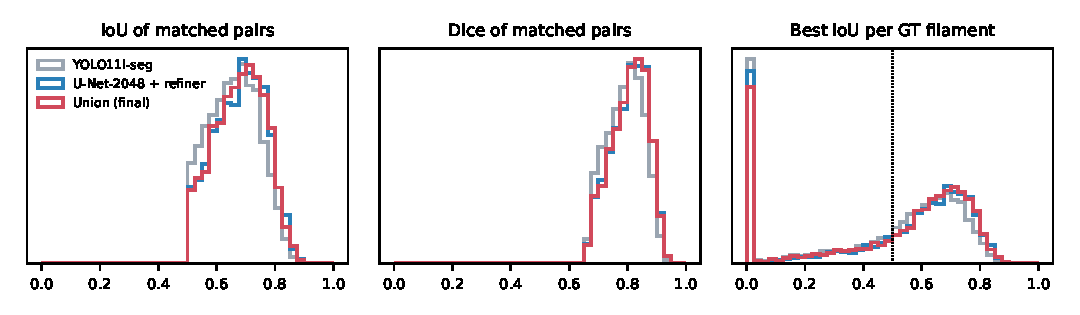
\includegraphics[width=0.85\textwidth]{fig_distributions.pdf}
  \caption{Distributions over all 707 OOF images and all annotation sets for YOLO alone, the refined
    U-Net-2048 and the final union. Left, middle: IoU and Dice of matched pairs. Right: best IoU of each
    ground-truth filament with any prediction (left of the dotted line: missed).}
  \Description{Three histograms comparing matched IoU, matched Dice and best IoU per ground-truth filament for three systems.}
  \label{fig:dist}
\end{figure*}

\subsection{Results}
    Table~\ref{tab:main} compares the stages. The refiner is the largest gain, +0.037 PQ over YOLO alone
    (paired 95\% CI +0.033 to +0.042), and comes mostly from recognition: its quality head discards false
    positives that YOLO's confidence cannot separate, so precision rises from 0.669 to 0.726 while recall
    also improves (0.605 to 0.622). The merge with the second source adds recall (0.622 to 0.653) at a small
    cost in precision. Its gain over YOLO + refiner is small, +0.002 (paired CI $-0.002$ to $+0.006$), but
    consistent: it helps on 4 of 5 folds (Table~\ref{tab:fold}), and it beats the refined U-Net-2048 alone
    by +0.008 (CI +0.004 to +0.012). Across folds the final PQ is $0.460 \pm 0.011$ (mean $\pm$ std).
    Fragmentation and over-merging stay below 4\% at every stage; the merge raises fragmentation slightly
    (1.2\% to 2.4\%) because a U-Net component can cover part of a filament that a YOLO instance also
    covers. Every system exceeds the human agreement level because it is scored against all annotators and
    predicts the filaments most of them draw. On the public leaderboard the final system scores 0.40
    (YOLO alone 0.35), against 0.37 for the two-stage YOLO11m + UNet++ solution~\cite{ghosh2026twostage}.

\begin{table}[t]
  \centering
  \caption{OOF PQ per fold.}
  \label{tab:fold}
  \resizebox{\columnwidth}{!}{%
  \begin{tabular}{lcccc}
    \toprule
    Fold ($n$) & YOLO & + refiner & U-Net-2048 & Union \\
    \midrule
    0 (142) & 0.417 & 0.452 & 0.435 & \textbf{0.456} \\
    1 (142) & 0.420 & \textbf{0.458} & 0.449 & 0.453 \\
    2 (141) & 0.405 & 0.444 & 0.448 & \textbf{0.450} \\
    3 (141) & 0.427 & 0.474 & 0.470 & \textbf{0.477} \\
    4 (141) & 0.434 & 0.462 & 0.455 & \textbf{0.463} \\
    \midrule
    Mean $\pm$ std & $0.421 \pm 0.011$ & $0.458 \pm 0.011$ & $0.451 \pm 0.013$ & $0.460 \pm 0.011$ \\
    \bottomrule
  \end{tabular}}
\end{table}

\begin{table}[t]
  \centering
  \caption{Ablations. Top: fold 0 (142 images, settings tuned on fold 0). Bottom: pooled 707-image OOF.}
  \label{tab:abl}
  \resizebox{\columnwidth}{!}{%
  \begin{tabular}{lcc}
    \toprule
    Variant & OOF PQ & Public \\
    \midrule
    U-Net alone (stage 2) & 0.406 & \\
    YOLO11l-seg alone & 0.417 & 0.35 \\
    \quad + refiner, 30 epochs, hflip TTA & 0.446 & \\
    \quad + endpoint-bridging fusion & 0.447 & 0.40 \\
    MeshNet refiner (7.5k params) & 0.448 & \\
    ResNet-34 refiner, 60 epochs, D4 & 0.456 & \\
    \quad + MeshNet ensemble, 6-model proposals & 0.457 & 0.39 \\
    \midrule
    YOLO + refiner (6-refiner vote) & 0.458 & 0.39 \\
    \quad U-Net maps trained 50 instead of 30 epochs & 0.458 & \\
    \quad + own U-Net proposals ($w=0.25$) & 0.442 & \\
    U-Net-2048 + refiner alone & 0.452 & 0.39 \\
    YOLO + refiner + U-Net-2048, $w=1.0$ & 0.451 & \\
    YOLO + refiner + U-Net-2048, $w=0.25$ (final) & \textbf{0.460} & \textbf{0.40} \\
    \bottomrule
  \end{tabular}}
\end{table}

\subsection{Ablations}
    Table~\ref{tab:abl} lists the variants we tried. Bridging broken filaments by their skeleton endpoints
    adds only 0.001 once the refiner is in, because splitting is already rare. Training the U-Net longer
    improved its own PQ on every fold but did not move the final PQ: the refiner, not its guidance maps, is
    the bottleneck. Proposals cut from our own 1024 px U-Net hurt (0.442): they overlap the YOLO proposals the
    refiner already sees and mostly add false positives. The native-resolution U-Net errs differently, and
    at a quarter of the YOLO weight its refined instances fill gaps without displacing better masks; at
    equal weight they do (0.451). A low weight needs a low score threshold (0.1); a high weight cannot recover the loss at any
    threshold from 0.05 to 0.3.



\subsection{Mask quality}
    Refinement shifts the whole distribution of matched IoU upward for both proposal sources
    (Figure~\ref{fig:dist}): the median rises from 0.662 for YOLO alone to 0.685 for both the refined
    U-Net-2048 and the final union (Dice 0.796 to 0.813). The two refined systems draw masks of the same
    quality and differ in how many filaments they find: 5,024 matched pairs for YOLO, 5,332 for the refined
    U-Net-2048 and 5,435 for the union, and the share of ground-truth filaments that no prediction covers at
    IoU $>0.5$ falls from 38.7\% to 35.0\% and 33.7\%. Most remaining misses have no overlapping prediction
    at all (the spike at 0), so they are detection failures rather than boundary errors.

\subsection{Efficiency}
    On Kaggle (2$\times$ T4), one YOLO fold model trains in 1.5~h, one U-Net fold in about 1~h and one
    refiner in 72~min. At test time the six refiners with D4 views take 3.4~s per image on a T4; the six YOLO
    models take about 5~s per image (on an RTX A2000, with mask voting on CPU); the merge runs on CPU.

\subsection{Strengths, weaknesses and improvements}
    The cascade splits the problem cleanly: the refiner raises both mask quality and precision, the second
    source raises recall, and both gains hold across folds. Fragmentation and over-merging stay low without
    a dedicated topology stage. The main weakness is recall (0.65): faint filaments that only some annotators
    draw are missed entirely, and the gain of the second source, though consistent, is within its
    uncertainty. OOF PQ also exceeds public PQ by about 0.06 for every model we submitted; test images come
    slightly more often from 2019--2022 (12\% against 9\%), years on which OOF PQ is lowest (0.36), but this
    explains only about 0.005, and public notebooks report a similar gap. Promising next steps are training
    the proposers for recall on low-agreement filaments, training one refiner on both proposal sources, and
    learning the merge instead of fixing $w$.

% ==================================== %
%            ACKNOWLEDGMENT            %
% ==================================== %
\section{Acknowledgment}\label{sec:acknowledgment}
    % Do not change
    The organization of the Filament Segmentation Challenge 2026 is partially supported by the U.S. National Science Foundation (NSF) under Grant No. 2209912 and 2433781, directorate for Computer and Information Science and Engineering (CSE), and Office of Advanced Cyberinfrastructure (OAC), and Grant No. 2511630, AST Division Of Astronomical Sciences and MPS Directorate for Mathematical and Physical Sciences.

    The Filament Segmentation Challenge 2026 is sponsored by the U.S. National Science Foundation (NSF) National Solar Observatory (NSO). 

    This work utilizes GONG data obtained by the NSO Integrated Synoptic Program, managed by the National Solar Observatory, which is operated by the Association of Universities for Research in Astronomy (AURA), Inc. under a cooperative agreement with the National Science Foundation and with contribution from the National Oceanic and Atmospheric Administration. The GONG network of instruments is hosted by the Big Bear Solar Observatory, High Altitude Observatory, Learmonth Solar Observatory, Udaipur Solar Observatory, Instituto de Astrofísica de Canarias, and Cerro Tololo Interamerican Observatory.

\bibliographystyle{ACM-Reference-Format}
\bibliography{main}

\end{document}
